\section{Results}
\begin{frame}[fragile]{Results: Driving Task} 
\begin{center}
 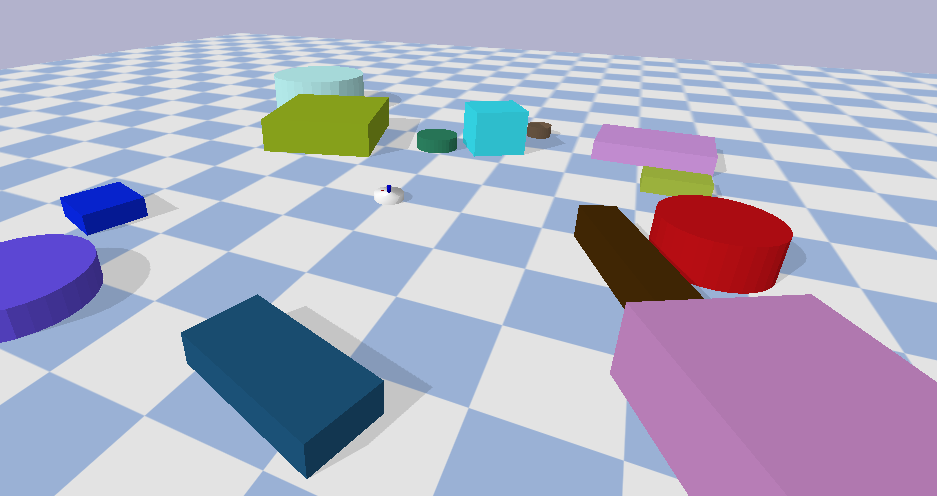
\includegraphics[width=0.8\textwidth]{figures/results/random1}
\end{center}
\end{frame}

\begin{frame}[fragile]{Results: Driving Task} 
\begin{center}
 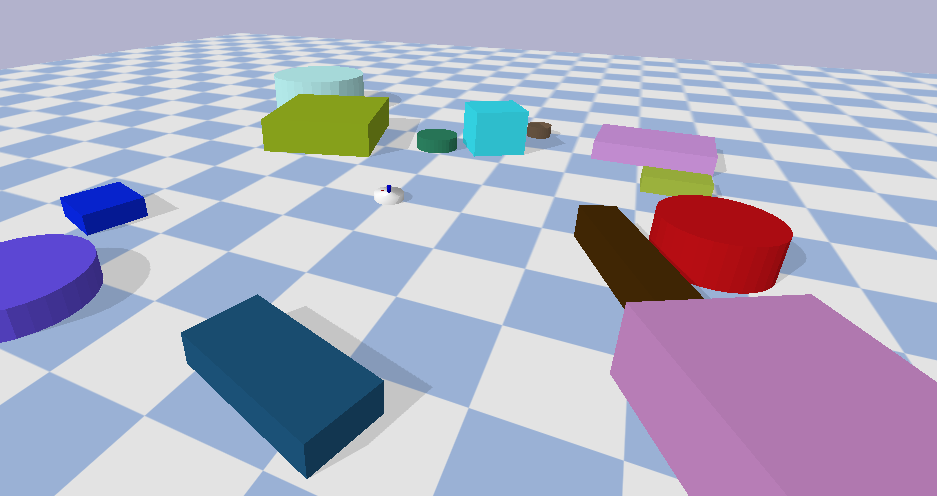
\includegraphics[width=0.8\textwidth]{figures/results/random1}
\end{center}
\end{frame}

\begin{frame}[fragile]{Results: Driving Task} 
  Reshuffle the environment
\begin{figure}
  \centering
  \subfloat{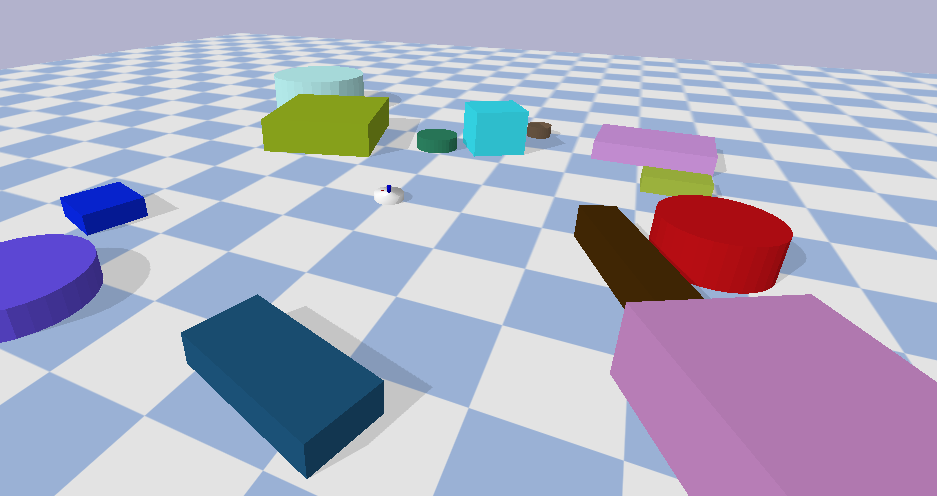
\includegraphics[width=0.48\textwidth]{figures/results/random1}}\quad
  \subfloat{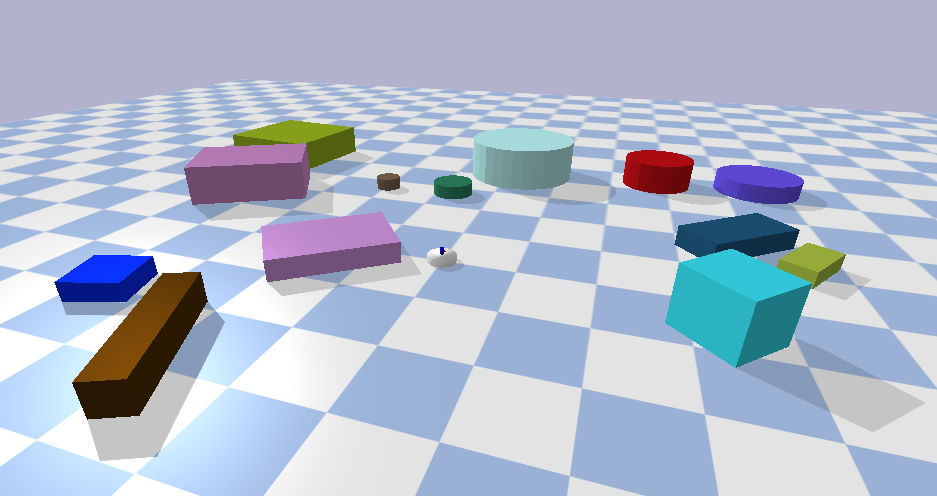
\includegraphics[width=0.48\textwidth]{figures/results/random2}}
\end{figure}
\end{frame}

% \begin{frame}[fragile]{Results} 
%   \begin{center}
%     \movie[width=0.8\textwidth, height=0.41\textwidth, autostart, poster]{}{figures/results/confetti.mp4}
%   \end{center}
% \end{frame}

\begin{frame}[fragile]{Results: Driving Task} 
\begin{table}[H]
    \centering
    \begin{tabular}%
    {l | p{0.3cm} p{0.3cm} p{0.3cm} p{0.3cm} p{0.3cm} p{0.3cm} p{0.3cm} p{0.3cm}p{0.3cm} p{0.3cm}}
  Run &  &   &  &  & Task &  &  &  &  & \\ \hline
  $\mathit{run}_1$ & 1 & 1  & 1 & 1 & 1 & 1 & 1 & 1 & 1 & 1\\
  $\mathit{run}_2$ & 1 & 1  & 1 & 1 & 1 & 1 & 1 & 1 & 1 & 1\\
  \quad\vdots &\vdots & \vdots  & \vdots & \vdots & \vdots & \vdots & \vdots & \vdots & \vdots & \vdots\\
  $\mathit{run}_{10}$ & 1 & 1  & 1 & 1 & 1 & 1 & 1 & 1 & 1 & 1\\\hline
    Total Tasks& 10 & 10  & 10 & 10 & 10 & 10 & 10 & 10 & 10 & 10\\
    Total Subtasks & 30 & 30  & 30 & 30 & 30 & 30 & 30 & 30 & 30 & 30\\\hline
    Tasks in experience & 0 & 1 & 2 & 3 &4 & 5 &6 & 7& 8  &9\\ 
    \end{tabular}
\end{table}\pause

\[\textrm{number of subtasks} = 10 * 10 * 3 = 300\]
\end{frame}


\begin{frame}[fragile]{Results: Driving task} 
Boxplot of 10 runs with random selection of (\textit{controller}, \textit{model})
\vspace{-1cm}
\begin{center}
  \hbox{\hspace{-0.7cm} 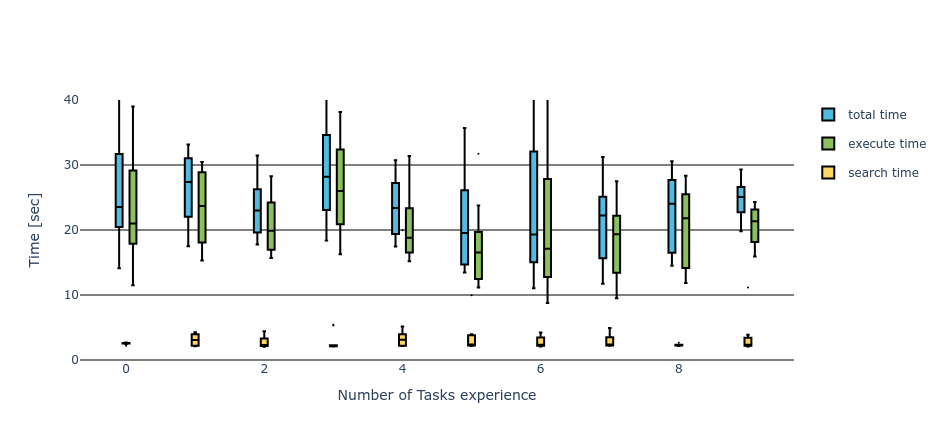
\includegraphics[width=1.05\textwidth]{figures/results/random_drive_time_no_k-graph} }
\end{center}
\end{frame}

\begin{frame}[fragile]{Results: Driving task} 
Boxplot of 10 runs with K-Graph action suggestions
\vspace{-1cm}
\begin{center}
  \hbox{\hspace{-0.7cm} 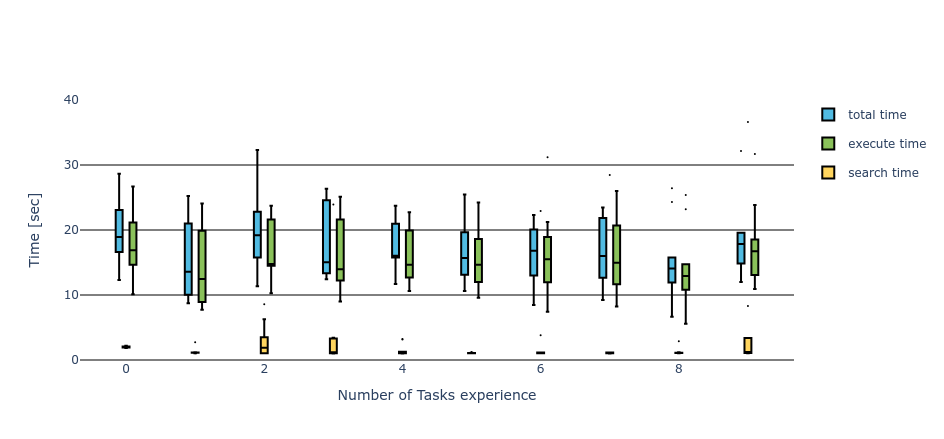
\includegraphics[width=1.05\textwidth]{figures/results/random_drive_time_k-graph} }
\end{center}
\end{frame}

\begin{frame}[fragile]{Results: Driving task} 
\begin{center}
  \begin{figure}
  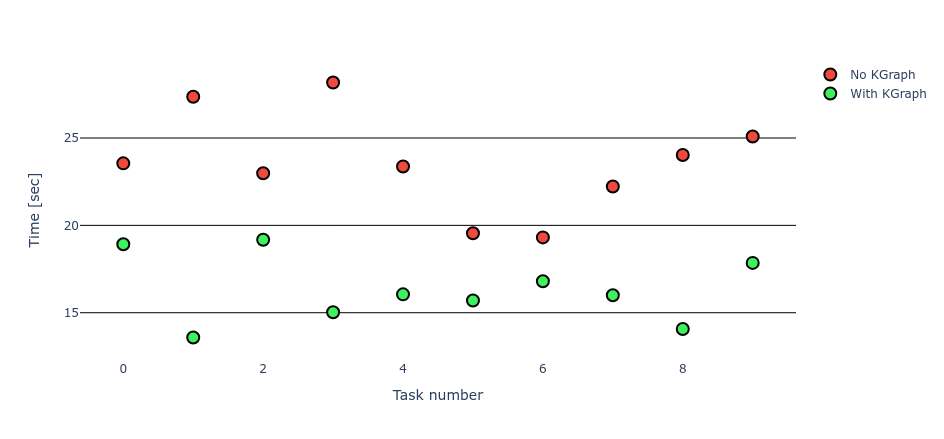
\includegraphics[width=0.8\textwidth]{figures/results/random_drive_time_vs}
  \caption{Median of 10 runs of drive task}
  \end{figure}
\end{center}
\end{frame}

\begin{frame}[fragile]{Results: Driving task} 
\begin{center}
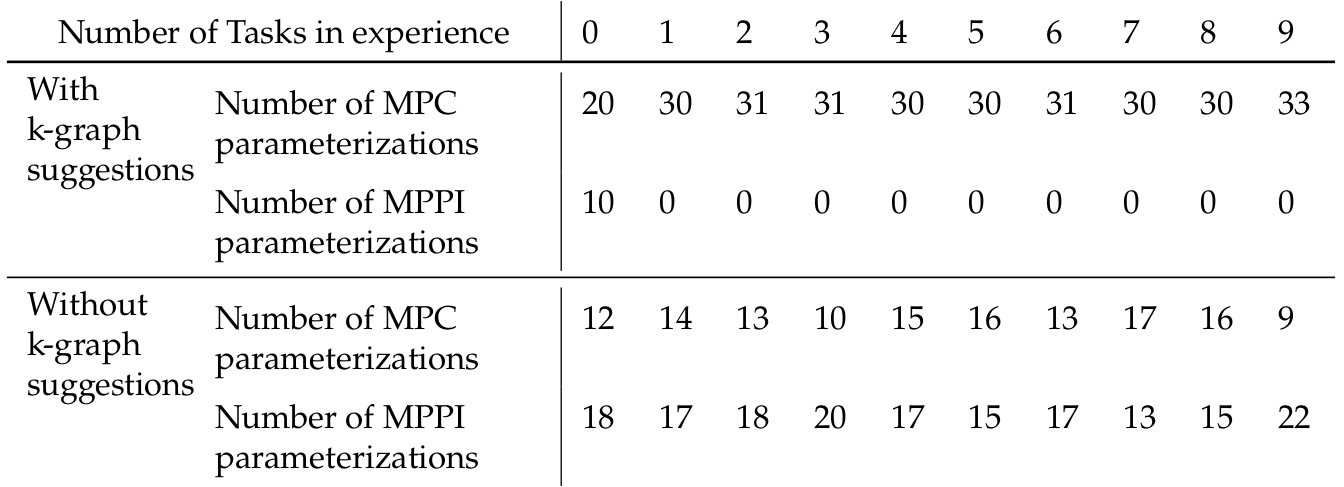
\includegraphics[width=1.0\textwidth]{figures/results/random_drive_para}
\end{center}
\end{frame}

\begin{frame}[fragile]{Results: Pushing task} 
\begin{center}
   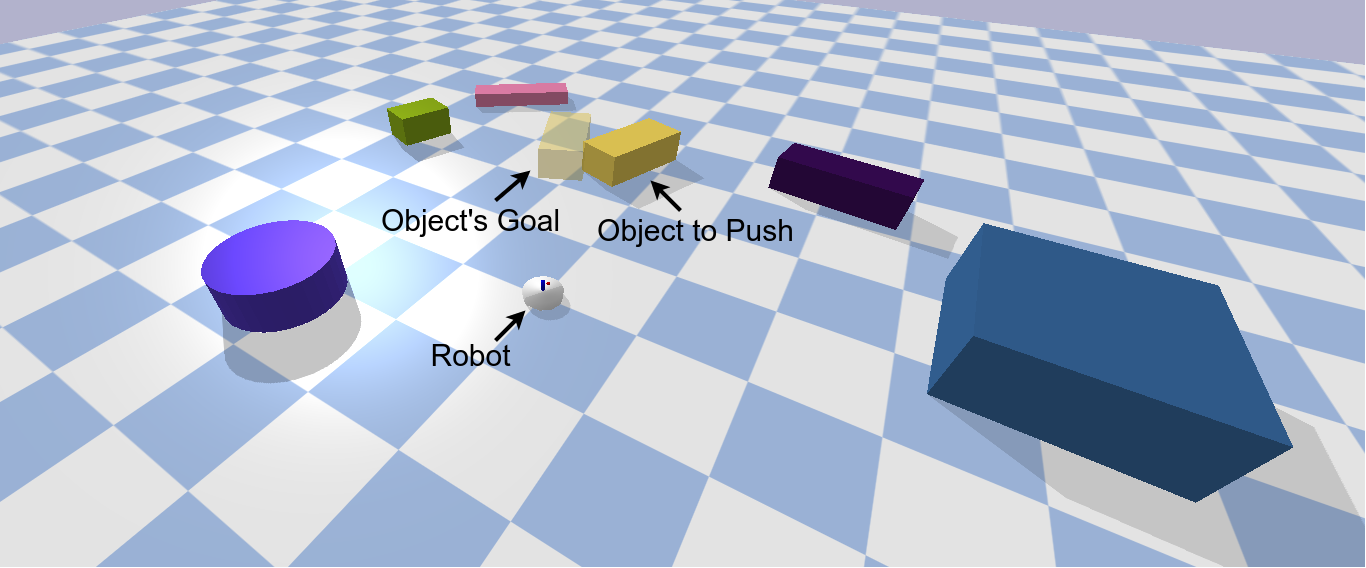
\includegraphics[width=1.0\textwidth]{figures/results/random_1.drawio}
\end{center}

\vspace{-1cm}
\[\textrm{number of subtasks} = 10 * 6 * 1 = 60\]
\end{frame}


\begin{frame}[fragile]{Results: Pushing task} 

\begin{center}
  \begin{figure}[H]
      \centering
 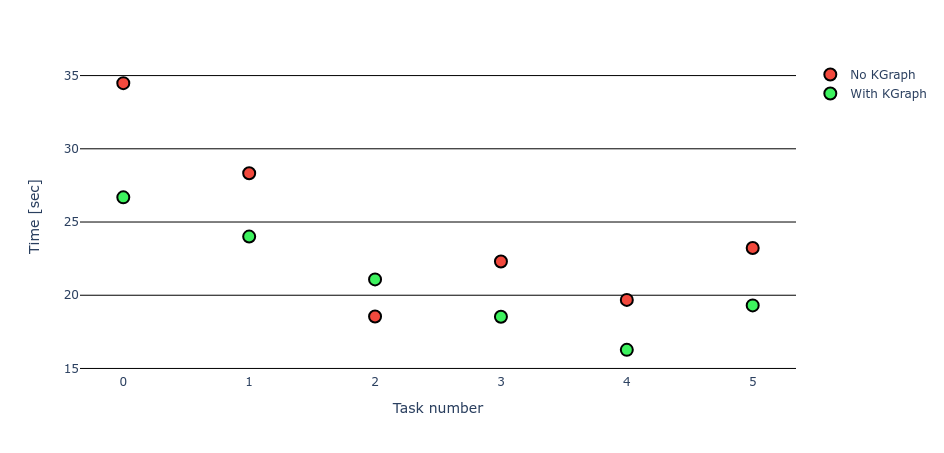
\includegraphics[width=0.9\textwidth]{figures/results/random_push_time_vs}
  \caption{Median of 10 runs to complete pushing tasks}
  \end{figure}
\end{center}
\end{frame}


% \begin{frame}[fragile]{Results: Pushing task} 
  % \todo{success factor targets the prediction error, not really that otehr thingy}
% \end{frame}

\begin{frame}[fragile]{Results: Pushing task} 
  \vspace{-1cm}
\begin{center}
  \begin{figure}[H]
      \centering
   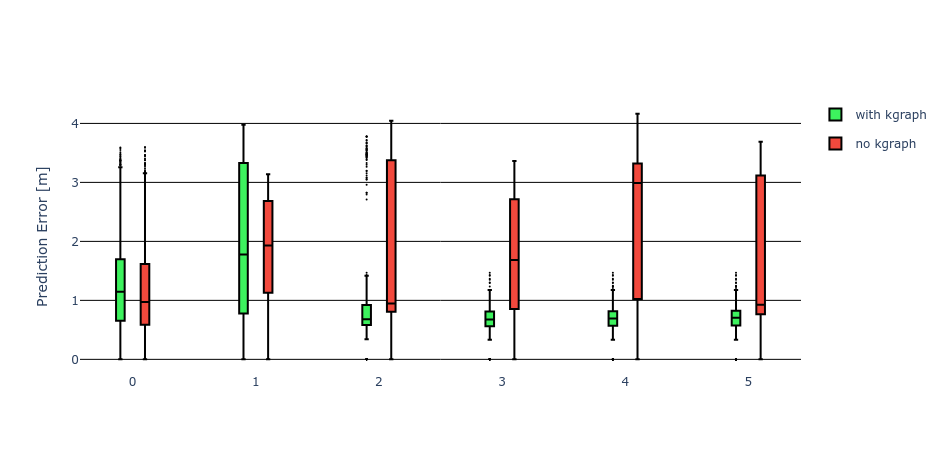
\includegraphics[width=0.9\textwidth]{figures/results/random_push_pe_vs}
  \caption{Median of 10 runs of pushing task}
  \end{figure}
\end{center}
\end{frame}

\begin{frame}[fragile]{Results: Pushing task} 
\begin{center}
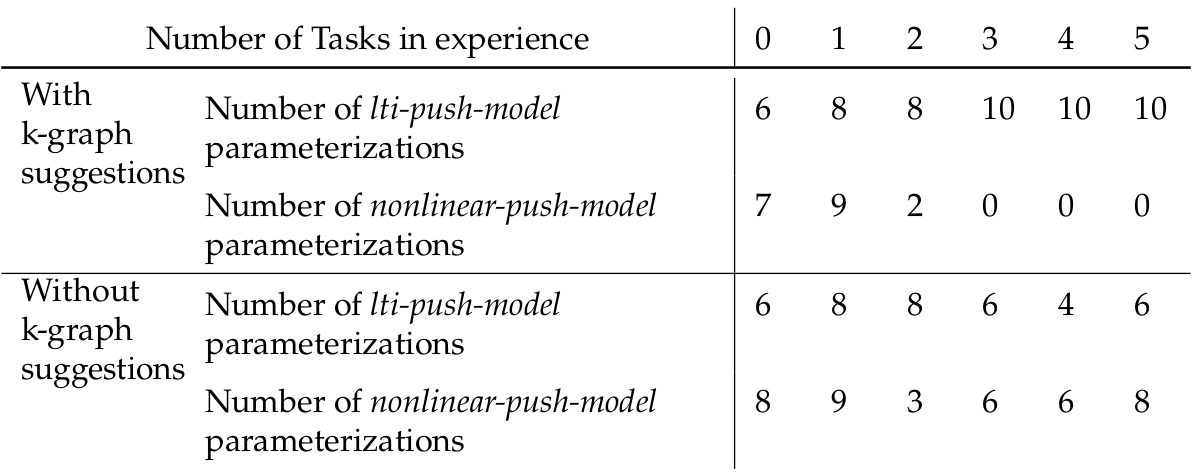
\includegraphics[width=1.0\textwidth]{figures/results/random_push_para}
\end{center}
\end{frame}


\begin{frame}[fragile]{Results} 
\begin{center}
 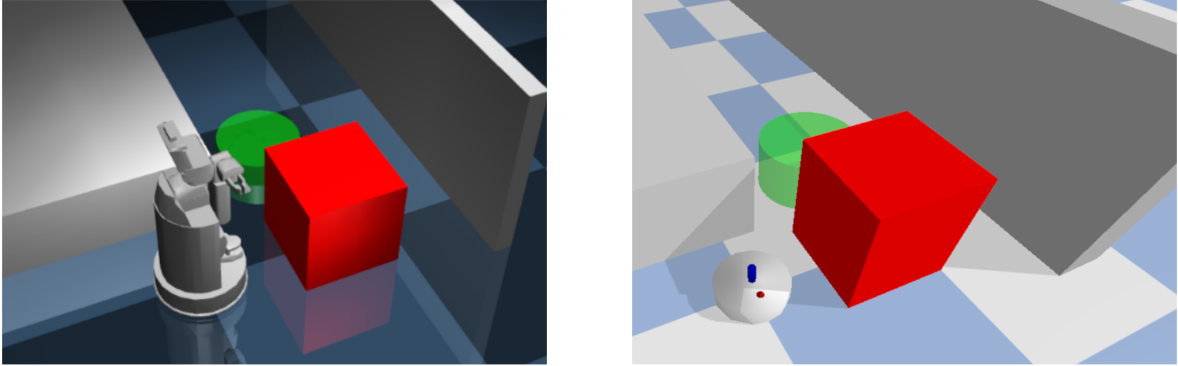
\includegraphics[width=1.0\textwidth]{figures/results/compare_sota}
\end{center}
\end{frame}


\begin{frame}[fragile]{Results} 
\begin{center}
 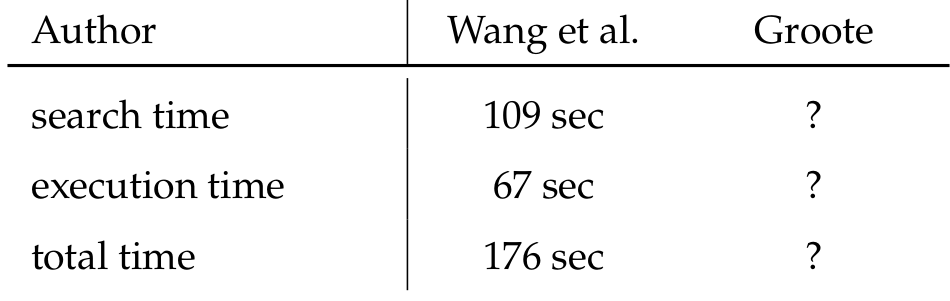
\includegraphics[width=0.7\textwidth]{figures/results/wang_groote_1}
\end{center}
\end{frame}

\begin{frame}[fragile]{Results} 
\begin{center}
 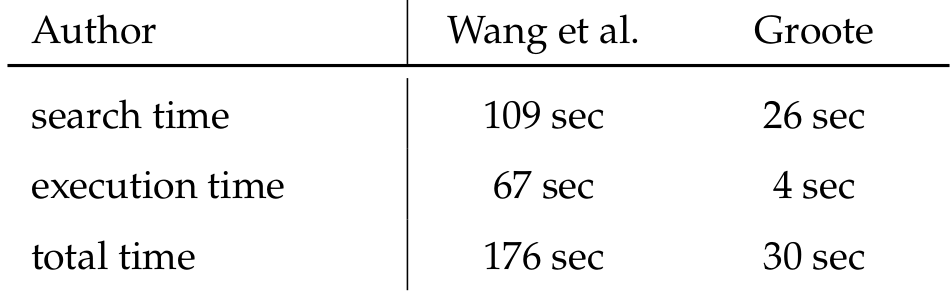
\includegraphics[width=0.7\textwidth]{figures/results/wang_groote_4}
\end{center}
\end{frame}





